\documentclass[twocolumn,10pt]{ltjsarticle}

\usepackage[top=20mm,bottom=20mm,left=25mm,right=25mm,columnsep=10mm]{geometry}
\usepackage[haranoaji,nfssonly]{luatexja-preset}
\usepackage{graphicx}
\usepackage{titlesec}
\usepackage{url}

\usepackage{multirow}    % セル結合用
\usepackage{tabularx}    % 表用&カラムサイズ指定

%% カラムサイズの指定用 %%
\newcolumntype{C}[1]{>{\centering\arraybackslash}p{#1}}
\newcolumntype{L}[1]{>{\raggedright\arraybackslash}p{#1}}
\newcolumntype{R}[1]{>{\raggedleft\arraybackslash}p{#1}}

\title{【実験】LombScargleピリオドグラムによるBOS2016の解析}
\author{山下 尚彦}
\date{\today}

\begin{document}
\maketitle

\section{はじめに}
私の卒業研究ではボットとなったPCを特定するために, ネットワーク上の通信を収集し, 
ボットとC2サーバ間の通信を解析する手法を提案した. 
卒業研究時の実験ではShinoBotを用いてボットとC2サーバの通信を擬似的に再現したが, 今回はBOS2016を用いて, 
通信をLomb-Scargleピリオドグラムで解析し, 通信の周期性を測定した. 

\section{BOS2016について}
今回の実験で使用するBOS2016は, 総務省実証事業「サイバー攻撃解析・防御モデル実践演習の実証実験の請負」にて実施し, 
研究者コミュニティから提供された組織内ネットワークへの侵害活動を観測されたデータセット\cite{マルウェア対策研42:online}
であり, マルウェア検体のハッシュ値情報や, 通信観測データ, プロセス観測データの他に, Windowsのイベントログや
ファイアウォールのログのデータを保持している. \\
マルウェアの検体は以下の表\ref{tab:bos2016}からわかるように, 動作が確認され通信が発生し, 攻撃の観測ができたものから, 
動作が確認されC2サーバへのSYNパケットのみが送信された検体, C2サーバとの通信を確認できなかったもの, 
検体の実行ができず通信が発生しなかったものがある. 
また, 攻撃活動を観測した検体(表\ref{tab:bos2016}のe04)の通信観測データについてはデータセットに含まれていない.

\begin{table}[htb]
    \centering
    \caption{BOS2016の検体の挙動と通信について}

    \begin{tabular}{C{2cm}L{1.5cm}L{2.8cm}}
        %% カラム名 %%
        \hline
        観測データ\par ディレクトリ & 挙動 & 通信 \\
        \hline \hline
        %% データ %%
        e04 & 動作 & 攻撃活動を観測 \\ \hline
        e12\par e20 & 動作 & C2サーバとの通信が成立しない(403, 404, 503) \\ \hline
        e43 & 実行不可 & 通信発生せず \\ \hline
        e70\par e435 & 動作 & C2サーバへSYNパケットのみ送信 \\
        \hline
    \end{tabular}
    \label{tab:bos2016}
\end{table}

\section{実験}
\subsection{解析手順}
まず, ネットワーク上の通信を観測したファイル(PCAPファイル)から以下の情報を抽出して,
解析に不要な情報を排除する. 

\begin{itemize}
    \item 通信時間のタイムスタンプ
    \item 送信元IPアドレス
    \item 受信先IPアドレス
\end{itemize}

次に,送信元IPアドレスと受信先IPアドレスのペアになるように通信データを分け, 
Lomb-Scargleピリオドグラムで周波数解析を行う. 

\subsection{周期性の測定方法}
Lomb-Scargleピリオドグラムによる信号の周期性はピークを用いることで判断することができる. 
これは, 信号が周期性のない正規分布だという過程に基づいて, 
ある値以上のピークを解析結果が示した場合に周期性があると判断される. 
次に送信元IPアドレス毎にグループ化し, さらに送信元IPアドレス内で受信先IPアドレスでグループ化する. ある確率が0.1\%以上, 
こうすることで送信元と受信先のIPアドレスのペア毎に通信を分けることができたので, 
これをつまり99.9\%周期的であるためには, 図のグラフのピークが0.18631798(${=P_{0.1}}$)以上であることを意味する. 
このグラフのピークは0.9993959064009751と, ${P_{0.1}}$を超えているため99.9\%以上周期的であると言える. 

\begin{figure}[htb]
    \centering
    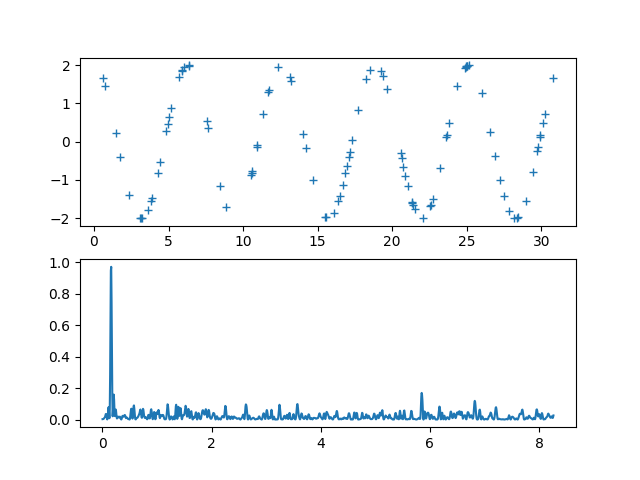
\includegraphics[width=8cm]{images/【実験】LombScargleピリオドグラムによるBOS2016の解析/lombscargle.png}
    \caption{欠損のある正弦波と解析結果}
    \label{fig:lombscargle}
\end{figure}

\subsection{実験データ}
BOS2016のうち, 通信観測データのなかったのe04以外の検体のデータを上記で述べた手順で解析し, 
周期性の測定を行った. 次の章で実験結果について述べる. 

\section{結果}
以下の表\ref{tab:result}は, e12, e20, e43, e70, e435それぞれの
送信IPアドレス数(表\ref{tab:result}のsrc), 
送信元と受信先IPアドレスのペア数(表\ref{tab:result}のpair), 
通信が周期的でない確率が0.5\%以下のペア数(表\ref{tab:result}の${P_{0.5}}$), 
通信が周期的でない確率が0.1\%以下のペア数(表\ref{tab:result}の${P_{0.1}}$), 
通信が周期的でない確率が0.01\%以下のペア数(表\ref{tab:result}の${P_{0.01}}$)
をまとめた表である.  \\
eXXはe12, e20, e43, e70を, eXXXはe435で実行した検体の通信を含めた全体のネットワークを観測したデータである. 
実験の結果, 全体のペア数と比べて${P_{0.01}}$のペア数は8分の1以下に絞り込むことができた. 

\begin{table}[htb]
    \centering
    \caption{BOS2016の実験結果}

    \begin{tabular}{C{8mm}L{8mm}L{8mm}L{8mm}L{8mm}L{8mm}L{8mm}}
        %% カラム名 %%
        \hline
        {} & src & pair & ${P_{0.5}}$ & ${P_{0.1}}$ & ${P_{0.01}}$ \\
        \hline \hline
        %% データ %%
        eXX  & 410 & 1183 & 152 & 94 & 65 \\
        e12  & 32  & 63   & 0   & 0  & 0  \\
        e20  & 12  & 23   & 0   & 0  & 0  \\
        e43  & 22  & 42   & 2   & 2  & 1  \\
        e70  & 24  & 49   & 11  & 10 & 6  \\
        eXXX & 217 & 550  & 107 & 73 & 57 \\
        e435 & 20  & 39   & 1   & 1  & 1  \\
        \hline
    \end{tabular}
    \label{tab:result}
\end{table}

\section{考察}
e12とe20を実行した機器ではC2サーバとの通信が成立していないため, 周期的な通信は観測されなかった. 
また, e43では検体を実行できなかった機器で周期的な通信を誤検知してしまったが, IPアドレスのペアが42ある内の1だったため
それほど影響はないと思われる. 
e70, e435はC2サーバに周期的にSYNパケットのみを送信していたため, 実験によってボットとC2サーバを検知することができた. \\
また, 今回の実験では確率を0.5\%, 0.1\%, 0.01\%と設定していたが, ペアの数が少なかったのが原因なのか, 
それほど絞り込むことができなかったように見える. 
実用的なことを考えると, さらに検証を続けて値を決定する必要があると考えられる. 

\section{おわりに}
本実験メモではLomb-Scargleピリオドグラムを用いてBOS2016を解析し, 周期性の測定を行った. 
実験の結果, ネットワークの通信を観測したデータから周期的な通信を検出することができ, 誤検知に関しても
それほど影響はないと考えられる. 
今回のデータセットでは攻撃活動を観測した機器の通信データがなかった. 
攻撃命令の通信は周期的な通信ではないため, これがどのように影響するのか今後実験などを行いたいと思う. 

\bibliographystyle{junsrt}
\bibliography{DB}
\end{document}